\documentclass[12pt]{article}

\usepackage[margin=1in]{geometry}
\usepackage[T1]{fontenc}
\usepackage{lmodern}
\usepackage{amsmath,amssymb,amsthm,bm}
\usepackage{booktabs,multirow,array}
\usepackage{graphicx}
\usepackage{algorithm}
\usepackage{algpseudocode}
\usepackage[numbers,sort&compress]{natbib}
\usepackage[hidelinks]{hyperref}
\usepackage{setspace}
\usepackage{lineno}

\onehalfspacing
\linenumbers
\emergencystretch=2em

\newtheorem{theorem}{Theorem}
\newtheorem{proposition}{Proposition}
\newtheorem{lemma}{Lemma}
\theoremstyle{remark}
\newtheorem{remark}{Remark}
\newcommand{\T}{\mathsf{T}}
\newcommand{\bbeta}{\boldsymbol{\beta}}
\newcommand{\bI}{\mathbf I}
\newcommand{\bone}{\mathbf 1}
\newcommand{\Scal}{\mathcal S}
\newcommand{\Bcal}{\mathcal B}
\newcommand{\Mcal}{\mathcal M}
\newcommand{\Var}{\operatorname{Var}}

\title{Fed-GEE: Federated Generalized Estimating Equations for Multisite
Health Data, with an Application to Veterans' Health}
\author{Feier Chang\textsuperscript{1} and Soumik Purkayastha\textsuperscript{1,2}\thanks{Corresponding author: Soumik Purkayastha,
Department of Biostatistics and Health Data Science, School of Public Health,
University of Pittsburgh, Pittsburgh, PA 15261, USA. Email: soumik@pitt.edu}\\[6pt]
\small\textsuperscript{1}Department of Biostatistics and Health Data Science, School of Public
Health,\\ \small University of Pittsburgh, Pittsburgh, Pennsylvania, USA\\
\small\textsuperscript{2}Center for Healthcare Evaluation, Research, and Promotion (CHERP),\\
\small VA Pittsburgh Healthcare System, Pittsburgh, Pennsylvania, USA}
\date{}

\begin{document}
\maketitle

\noindent\textbf{Short title:} Small-site inference for federated GEE

\begin{abstract}
Joint analysis of multisite health data increases sample size, population
diversity, and generalizability. Yet patient records often cannot be pooled,
outcomes are correlated within sites, and sites are often few. We propose
federated generalized estimating equations (Fed-GEE) for population-averaged
associations. By exchanging site score vectors and information matrices, Fed-GEE
reproduces the pooled estimate exactly. With few sites as the independent
clusters, however, the sandwich variance is too small and normal critical values
are too narrow. We derive federated versions of the small-sample variance
corrections and reference distributions used in pooled analyses. We give
theoretical justification and a simulation-based recommendation: the
Kauermann--Carroll correction with Bell--McCaffrey degrees of freedom. In
simulations with 10 to 50 sites, Fed-GEE matched pooled GEE to numerical
precision, and the recommended procedure kept 95\% interval coverage near nominal
(0.929 to 0.971), compared with as low as 0.863 without correction.
Meta-analysis of site-specific fits covered as low as 0.010. We applied Fed-GEE
to 29{,}041 hospitalizations of 18{,}900 Veterans with alcohol use disorder,
emulating a federation of 18 Veterans Health Administration regional networks.
Clinician and non-clinician addiction consultation were each associated with
starting alcohol use disorder medication (odds ratios 1.47 and 1.88). These
findings match the pooled analysis, yet no patient records need leave their
sites. Non-clinician consultation was also five times as common (15.0\% versus
2.9\%). Where non-clinician staff cost less to hire, expanding this workforce
could increase consultation capacity within a fixed budget.
\end{abstract}

\noindent\textbf{Keywords:} sandwich variance estimator; small-sample
correction; few clusters; Bell--McCaffrey degrees of freedom; distributed
inference; alcohol use disorder; addiction consultation

\section{Introduction}
\label{sec:introduction}

Alcohol use disorder (AUD) is more common among US Veterans than in the general
adult population. National surveys estimated lifetime prevalences of 42.2\%
and 29.1\%, respectively \citep{fuehrlein2016burden,grant2015epidemiology}.
Among Veterans, AUD is associated with substantial psychiatric morbidity, suicidal behavior,
and higher all-cause mortality
\citep{fuehrlein2016burden,chwastiak2010association}.

Each hospitalization for AUD offers an opportunity to initiate
treatment \citep{joudrey2020inpatient}. Effective medications for AUD (MAUD)
are available but remain underused \citep{mason2022looking}. Hospital addiction
consultation services are associated with greater initiation of medications
for opioid use disorder \citep{danovitch2024addiction,ober2025hospital}.
Evidence for AUD is more limited, although recent studies suggest that
consultation may also support MAUD initiation
\citep{singhtan2023addiction,anderson2026initiation}.

Using national Veterans Health Administration (VHA) data, we examine whether
hospital addiction consultation is associated with higher MAUD initiation and
whether this association is present for consultation delivered by both
clinicians and non-clinicians. In this study, clinicians are physicians and
advanced practice clinicians; non-clinicians are social workers, nurses, and
peer support staff \citep{anderson2026initiation}. The latter can support
treatment engagement and coordination, with prescribing remaining the
responsibility of an authorized clinician. These associations can inform
staffing policy. Evidence confined to clinician consultation would favor
prioritizing clinician capacity; evidence for non-clinician consultation would
support considering a broader workforce. Where non-clinician staff are more
available and less costly to hire, this could expand consultation capacity
within a fixed budget.

We analyze 29{,}041 hospitalizations of 18{,}900 Veterans with a primary
diagnosis of AUD in 2022 or 2023 \citep{anderson2026initiation}. The outcome is
MAUD initiation during hospitalization or within 7 days of discharge.
Hospitalizations are clustered within Veterans and within regions that share
health services and practice patterns. Our policy target is the
population-averaged association between consultation and MAUD initiation across
the VHA. Generalized estimating equations (GEE) provide a routine way to
estimate this marginal association while allowing correlated outcomes
\citep{liang1986longitudinal,zeger1988models}.

The scientific setting adds a need to limit the movement of sensitive records.
Pooling patient-level data creates additional data-transfer and access risks,
and AUD diagnoses carry stigma that can itself discourage treatment seeking
\citep{rieke2020future,keyes2010stigma}. These concerns motivate a federated
system in which records remain under local control and sites exchange
statistical summaries. Federated methods for generalized linear mixed models
are available \citep{yan2023privacy}, but their conditional regression
coefficients do not directly answer our population-averaged question.
We therefore require a federated GEE procedure that supports both marginal
estimation and inference. Keeping records local reduces the need to share
sensitive data; formal protection against disclosure from exchanged summaries
requires additional safeguards \citep{kairouz2021advances}.

The VHA's regional organization creates a further inferential challenge. Its
18 Veterans Integrated Service Networks (VISNs) are administrative units
responsible for regional resources and policy. Shared staffing policies and
practice patterns motivate treating each VISN as an independent unit in our
analysis. Thus, despite the large number of hospitalizations, inference rests
on only 18 clusters. This does not prevent computation of the GEE point
estimate, but it can undermine the large-cluster approximations used for
inference, whether estimation is centralized or decentralized. With few
clusters, the usual sandwich variance tends to be biased downward and normal
Wald intervals can undercover
\citep{mancl2001covariance,kauermann2001note}. Established remedies include the
Kauermann--Carroll (KC), Mancl--DeRouen (MD), and Fay--Graubard (FG) variance
corrections and small-sample reference distributions
\citep{kauermann2001note,mancl2001covariance,fay2001small,bell2002bias,liredden2015sandwich}.
Their conventional formulations use observation-level residuals and cluster
leverage matrices that are directly available in a pooled analysis. Applying
them in a federation requires expressions that can be evaluated from shared
summaries. The reference distribution must likewise be determined from these
summaries, with critical values that reflect unequal information across the
small number of sites
\citep{bell2002bias,imbens2016robust}.

The contributions of this paper are as follows. We develop Fed-GEE for
population-averaged estimation and small-sample inference in federated networks,
with implementations both with and without a coordinating center. We express
the KC, MD, and FG variance corrections in score space, using site score
vectors and information matrices without transferring patient-level records.
We also compute coefficient-specific Bell--McCaffrey degrees of freedom from
these summaries, enabling federated construction of the $t$ reference
distributions used for confidence intervals and hypothesis tests. Both the
variance correction and reference distribution are computed in a single
post-convergence stage. With a coordinating center, this requires one additional
exchange of site summaries; without a center, the summaries are aggregated
through neighbor consensus. Under an
affine working-score model with covariance correct up to scale, we show that
the KC half-power gives an exactly unbiased variance estimator and is the
unique exponent in the proposed family with this property. Extensive
simulations examine coverage with 10 to 50 sites and unequal site sizes, and
additional simulations assess decentralized fitting with an uncorrected
sandwich. The decentralized small-sample correction is developed theoretically
and is not evaluated in these simulations.
Finally, we apply the procedure to the VHA staffing question. The application
uses centrally available records to emulate federation across VISNs and verify
the results against a pooled analysis.

Section~\ref{sec:methods} presents the VHA analysis model, federated GEE,
score-space corrections, and reference distributions, followed by algorithms
with and without a coordinating center. Section~\ref{sec:simulation} reports
the simulation study, and Section~\ref{sec:application} presents the VHA
application. Section~\ref{sec:discussion} discusses implications and limitations.

\section{Methods}
\label{sec:methods}

\subsection{Application model and estimand}
\label{sec:data}

For hospitalization $t$ of Veteran $j$ in VISN $i$, let $Y_{ijt}$ indicate MAUD
initiation within the outcome window defined above. We specify the marginal
logistic model
\begin{equation}
\operatorname{logit}\{\Pr(Y_{ijt}=1\mid C_{ijt},N_{ijt},Z_{ijt})\}
=\beta_0+\beta_C C_{ijt}+\beta_N N_{ijt}+Z_{ijt}^{\T}\boldsymbol\gamma,
\label{eq:applicationmodel}
\end{equation}
where $C_{ijt}$ and $N_{ijt}$ indicate clinician and non-clinician consultation,
respectively, with no consultation as the reference. The nine adjustment
covariates in $Z_{ijt}$ account for measured differences in case mix and
hospital care. They cover demographics (age at least 65 years and female sex),
alcohol severity and co-occurring substance use (no or low AUDIT-C score and
opioid use disorder), medical complexity (Care Assessment Need score at or above
the 60th percentile, mild or worse frailty, and intensive care unit stay), and
hospital processes (psychiatry discharging service and discharge against
medical advice) \citep{anderson2026initiation}. These groups correspond to those
in Figure~\ref{fig:forest}.

We fit the model by GEE with working independence and $p=12$ coefficients.
Hospitalizations are nested within Veterans and Veterans within VISNs; the VISN
is both the unit of federation and the independent unit for variance estimation.
The target estimands, $\exp(\beta_C)$ and $\exp(\beta_N)$, are adjusted
population-averaged odds ratios for each consultation type relative to no
consultation. They describe associations, not causal effects. The following
formulation extends this model to general outcomes and working covariances.

\subsection{Estimating equations and federated fitting}
\label{sec:fitting}

Suppose the data come from $K$ independent sites. Site $i$ holds $n_i$ patient
clusters, indexed by $j=1,\ldots,n_i$. Cluster $j$ has a response vector $Y_{ij}$,
a covariate matrix $X_{ij}$, and marginal mean
$\mu_{ij}(\bbeta)=g^{-1}(X_{ij}\bbeta)$ for a known link $g$ and a $p$-vector
$\bbeta$. Let $D_{ij}=\partial\mu_{ij}/\partial\bbeta^{\T}$, and let $V_{ij}$ be
a working covariance matrix \citep{liang1986longitudinal}. Each site computes a
score vector and an information matrix,
\begin{equation}
\Scal_i(\bbeta)=\sum_{j=1}^{n_i}D_{ij}^{\T}V_{ij}^{-1}
  \{Y_{ij}-\mu_{ij}(\bbeta)\},
\qquad
\Bcal_i(\bbeta)=\sum_{j=1}^{n_i}D_{ij}^{\T}V_{ij}^{-1}D_{ij}.
\label{eq:site}
\end{equation}
The GEE estimator $\widehat\bbeta$ solves
$\Scal(\bbeta)=\sum_i\Scal_i(\bbeta)=0$. Because the score and information
matrix are additive across sites, the estimating equation can be solved using
site summaries. At the current value $\bbeta^{(r)}$,
each site sends $\Scal_i\{\bbeta^{(r)}\}$ and $\Bcal_i\{\bbeta^{(r)}\}$ to a
coordinating center. The center adds them and takes a Fisher-scoring step,
\begin{equation}
\bbeta^{(r+1)}=\bbeta^{(r)}+\Bcal\{\bbeta^{(r)}\}^{-1}\Scal\{\bbeta^{(r)}\},
\qquad
\Bcal=\sum_{i=1}^K\Bcal_i.
\label{eq:update}
\end{equation}
It then returns $\bbeta^{(r+1)}$ to the sites. We stop when
$\|\bbeta^{(r+1)}-\bbeta^{(r)}\|<10^{-8}$, with at most 50 iterations. Each
message has $p+p(p+1)/2$ summary statistics, and no patient-level record leaves
a site. Algorithm~\ref{alg:fedgee} summarizes the fitting routine and the
one-shot post-convergence correction developed in Section~\ref{sec:correction}.


\subsection{Large-sample inference}
\label{sec:largeK}

Inference uses the cluster-robust sandwich variance at the site level,
\begin{equation}
\widehat V_{\mathrm{S}}=\widehat\Bcal^{-1}\widehat\Mcal\widehat\Bcal^{-1},
\qquad
\widehat\Mcal=\sum_{i=1}^K\widehat\Scal_i\widehat\Scal_i^{\T},
\label{eq:naive}
\end{equation}
where $\widehat\Scal_i=\Scal_i(\widehat\bbeta)$ and
$\widehat\Bcal=\sum_i\Bcal_i(\widehat\bbeta)$. The site is the independent unit
because patients within a site share practice patterns, staffing, and local
policy. The site-level sandwich accommodates dependence among patients within a site
and remains asymptotically valid under working-covariance misspecification,
provided the marginal mean is correctly specified and the sites are independent
\citep{liang1986longitudinal}. Suppose
the sites are independent, $p$ is fixed, $K^{-1}\widehat\Bcal\to B_0$, and
$K^{-1}\widehat\Mcal\to M_0$ in probability. Under the regularity conditions of
\citet{liang1986longitudinal}, $\widehat\bbeta$ is consistent and
\[
\sqrt K(\widehat\bbeta-\bbeta_0)\overset{d}{\longrightarrow}
N(0,B_0^{-1}M_0B_0^{-1})
\quad\text{as }K\to\infty.
\]
Hence $\widehat V_{\mathrm{S}}$ estimates $\Var(\widehat\bbeta)$ directly, and
Wald intervals use normal critical values. Web Appendix A states the conditions.
The result is standard, because $\widehat\bbeta$ is the pooled GEE estimator.

\subsection{The small-site problem}
\label{sec:smallK}

The large-sample approximation depends on the number of independent sites,
which can be small even in a large health-system cohort.
Estimating the regression coefficients from these same sites
constrains the fitted scores and can bias the sandwich variance downward.

Collect the fitted scores as the columns of
$S=[\widehat\Scal_1,\ldots,\widehat\Scal_K]\in\mathbb R^{p\times K}$. Since
$S\bone_K=0$ at the GEE solution,
\begin{equation}
\operatorname{rank}(\widehat\Mcal)\le\min(p,K-1).
\label{eq:rank}
\end{equation}
Thus, the meat is singular whenever $K\le p$ (Web Appendix E). For $K>p$,
the bound does not imply singularity, but the variance estimate still depends
on at most $K-1$ independent score contrasts.

Fitting also reduces the expected score variation under a correctly specified
affine working model. The reduction depends on each site's contribution to the
total information, so unequal information across sites can produce unequal
attenuation. This provides a working-model explanation for the downward bias
of the sandwich variance with few clusters
\citep{mancl2001covariance,kauermann2001note}. The score-space corrections below
account for this attenuation through site leverage; Section~\ref{sec:exact}
states the conditions under which the correction is exact.

\begin{remark}[Independent units in the VHA analysis]
\label{rem:vhaunits}
The VHA cohort contains 29{,}041 hospitalizations, but the site-level sandwich
is constructed from only 18 VISN scores. Additional hospitalizations can
increase information for estimation without increasing the number of
independent units available for variance estimation. With $p=12$ coefficients,
the rank bound does not force singularity, but neither the large cohort nor
$K>p$ ensures that the large-sample reference distribution is adequate.
\end{remark}

\subsection{Score-space correction and site leverage}
\label{sec:correction}
\label{sec:leverage}

Conventional small-sample corrections use observation-level residuals and
cluster leverages \citep{kauermann2001note,mancl2001covariance,fay2001small}.
In a federation, the coordinating center instead has access to
$\widehat\Scal_i$ and $\Bcal_i(\widehat\bbeta)$. We express the corrections
through these summaries, allowing variance estimation to be completed in one
additional exchange after convergence.

Define the information-standardized score and site leverage
\begin{equation}
z_i=\widehat\Bcal^{-1/2}\widehat\Scal_i,
\qquad
G_i=\widehat\Bcal^{-1/2}\Bcal_i(\widehat\bbeta)\widehat\Bcal^{-1/2}.
\label{eq:standardize}
\end{equation}
Each $G_i$ is symmetric and positive semidefinite, with $\sum_iG_i=\bI$ and
$\sum_i\operatorname{tr}(G_i)=p$. It measures site $i$'s contribution to the
total information and serves as the site leverage. For linear regression with
one observation per site and $V_{ij}=1$, $\operatorname{tr}(G_i)$ reduces to the
usual hat value $h_{ii}$. If all sites contribute equal information,
$G_i=\bI/K$; otherwise, leverage varies with site size and covariate
distribution. Web Appendix C establishes invariance to the choice of matrix
square root.

We require $\bI-G_i\succ0$ for every site, or equivalently
$\widehat\Bcal-\Bcal_i(\widehat\bbeta)\succ0$. The condition fails only if one
site alone identifies some direction of $\bbeta$. We report the smallest
eigenvalue of $\bI-G_i$ across sites as a diagnostic.

\subsection{Variance corrections}
\label{sec:three}

\emph{Kauermann--Carroll (KC) and Mancl--DeRouen (MD).} For an exponent
$\alpha>0$, let $A_i(\alpha)=(\bI-G_i)^{-\alpha}$ and
\begin{equation}
\widehat V(\alpha)=\widehat\Bcal^{-1/2}
\Big\{\sum_{i=1}^KA_i(\alpha)z_iz_i^{\T}A_i(\alpha)\Big\}
\widehat\Bcal^{-1/2}.
\label{eq:adjusted}
\end{equation}
The adjustment inflates each standardized score according to its site leverage.
The choice $\alpha=1/2$ is the score-space
analogue of the KC correction \citep{kauermann2001note}. The choice $\alpha=1$ is
the analogue of the MD correction \citep{mancl2001covariance}. We write
$\widehat V_{\mathrm{KC}}=\widehat V(1/2)$ and
$\widehat V_{\mathrm{MD}}=\widehat V(1)$.
\citet{kauermann2001note} chose the half-power so that the corrected variance is
unbiased in the linear model with a correct working covariance.
\citet{mancl2001covariance} derived the full power from a first-order bias
approximation. Under the working model of Section~\ref{sec:exact}, the full
power overestimates the variance (Theorem~\ref{thm:exact}). The adjustment acts
on the standardized score. Applying $(\bI-G_i)^{-\alpha}$ directly to the raw score
$\widehat\Scal_i$ gives a different estimator in general (Web Appendix B).

\emph{Fay--Graubard (FG).} \citet{fay2001small} rescale each cluster's score
by a diagonal factor. In score space the factor for site $i$ is
\begin{equation}
F_i=\operatorname{diag}\Big[\big\{1-\min\big(b,\,
(\Bcal_i\widehat\Bcal^{-1})_{kk}\big)\big\}^{-1/2}\Big]_{k=1}^p,
\qquad
\widehat V_{\mathrm{FG}}=\widehat\Bcal^{-1}
\Big(\sum_{i=1}^KF_i\widehat\Scal_i\widehat\Scal_i^{\T}F_i\Big)
\widehat\Bcal^{-1},
\label{eq:fg}
\end{equation}
with the default bound $b=0.75$. FG inflates each coordinate of the score
separately using the diagonal of the site's information share. The bound
limits inflation when information about a coefficient is concentrated in one
site.
\citet{liredden2015sandwich} found FG preferable to KC when cluster sizes vary
widely.

All three estimators share a common form. Write the corrected raw score as
$T_i\widehat\Scal_i$, with
$T_i=\widehat\Bcal^{1/2}A_i(\alpha)\widehat\Bcal^{-1/2}$ for KC and MD and
$T_i=F_i$ for FG. Then each estimator equals
\begin{equation}
\widehat V_T=\widehat\Bcal^{-1}
\Big(\sum_{i=1}^KT_i\widehat\Scal_i\widehat\Scal_i^{\T}T_i^{\T}\Big)
\widehat\Bcal^{-1}.
\label{eq:common}
\end{equation}
The uncorrected sandwich~\eqref{eq:naive} is the case $T_i=\bI$.

\begin{remark}[Relation to CR2]
With working independence and an identity link, $\widehat V_{\mathrm{KC}}$ equals
the bias-reduced linearization estimator CR2
\citep{bell2002bias,pustejovsky2018small}. For logistic GEE the two differ,
because the working weights are not constant. In the VHA application they
differed by less than 0.5\% (Section~\ref{sec:application}).
\end{remark}

\subsection{Exactness of the half-power}
\label{sec:exact}

The half-power in the KC correction is exact under a working model for the
scores. The model treats $\widehat\Bcal$ and the $\Bcal_i$ as fixed matrices
$B$ and $B_i$.

\begin{theorem}[Affine working-score exactness]
\label{thm:exact}
Conditionally on the design, suppose
$\Scal_i(\bbeta)=U_i-B_i(\bbeta-\bbeta_0)$, where the $B_i$ are fixed positive
semidefinite matrices, the $U_i$ are independent, $E(U_i)=0$, and
$\Var(U_i)=\tau B_i$ for some $\tau>0$. Suppose $B=\sum_iB_i\succ0$ and
$B-B_i\succ0$ for every $i$. Define $G_i$ and $z_i$ by
\eqref{eq:standardize} with $\widehat\Bcal$ replaced by $B$. Then
\[
E(z_iz_i^{\T})=\tau G_i(\bI-G_i),
\qquad
E\Big\{\sum_{i=1}^KA_i(\tfrac12)z_iz_i^{\T}A_i(\tfrac12)\Big\}=\tau\bI.
\]
Hence $\widehat V_{\mathrm{KC}}$ is unbiased for
$\Var(\widehat\bbeta)=\tau B^{-1}$ at every finite $K$. Within the family
$A_i(\alpha)$, $\alpha=1/2$ is the only exponent that is unbiased for all
admissible $\{B_i\}$. The choice $\alpha=1$ overestimates the variance.
\end{theorem}

The proof is given in Web Appendix B. Under the affine working model, the
half-power adjustment removes the attenuation in the expected outer product of
each standardized score. The condition $\Var(U_i)=\tau B_i$ requires the working
covariance to be correct up to a common scale, as in the original KC derivation
\citep{kauermann2001note}. The result establishes exactness and uniqueness of
the exponent within this family under that condition. For logistic GEE or a
misspecified working covariance, the correction is based on linearization;
its finite-sample performance is evaluated in Section~\ref{sec:simulation}.

\begin{remark}
As $K\to\infty$ with no dominant site, $\max_i\lambda_{\max}(G_i)\to0$ in
probability. Then $\widehat V_{\mathrm{KC}}$, $\widehat V_{\mathrm{MD}}$,
$\widehat V_{\mathrm{FG}}$, and $\widehat V_{\mathrm{S}}$ have the same
first-order limit (Web Appendix D). Their effects are therefore asymptotically negligible under these conditions.
\end{remark}

\subsection{Reference distribution}
\label{sec:df}

Small-sample inference also requires an appropriate reference distribution.
The Wald statistic
$(\widehat\beta_j-\beta_{j})/\widehat V_{jj}^{1/2}$ is compared with a
reference distribution, and the normal distribution is too light-tailed when $K$
is small \citep{liredden2015sandwich}. Common choices are the $t$ distribution
with $K-p$ or $K-1$ degrees of freedom
\citep{mancl2001covariance,cameron2015practitioner}. A fixed count does not
respond to unequal information across sites. We therefore use the
Satterthwaite approximation of \citet{bell2002bias}, computed in score space.

The variance estimator is constructed from a small number of site scores and
can remain highly variable after bias correction \citep{kauermann2001note}.
The Bell--McCaffrey degrees of freedom account for this variability by matching
the first two moments of the corrected variance under a working model. Equal
information across sites gives $K-1$ degrees of freedom; concentration of
information in fewer sites reduces the effective degrees of freedom and
increases the critical value.

Fix a coefficient $j$ and let $e_j$ be the $j$th unit vector. Define
$a_i=T_i^{\T}\widehat\Bcal^{-1}e_j$. By~\eqref{eq:common}, the corrected
variance of $\widehat\beta_j$ is
\[
\widehat V_{T,jj}=\sum_{i=1}^K(a_i^{\T}\widehat\Scal_i)^2.
\]
Under the working model of Theorem~\ref{thm:exact} with Gaussian $U_i$, this is
a quadratic form in the $U_i$. Its first two moments are determined by the
$K\times K$ matrix
\begin{equation}
C_{ik}=\mathbf 1\{i=k\}\,a_i^{\T}\Bcal_ia_i
-(\Bcal_ia_i)^{\T}\widehat\Bcal^{-1}(\Bcal_ka_k),
\qquad i,k=1,\ldots,K.
\label{eq:bmkernel}
\end{equation}
Matching these moments to a scaled $\chi^2$ distribution gives the degrees of
freedom
\begin{equation}
\nu_j^{\mathrm{BM}}=\frac{\{\operatorname{tr}(C)\}^2}{\operatorname{tr}(C^2)}.
\label{eq:bmdf}
\end{equation}
The interval for $\beta_j$ is
$\widehat\beta_j\pm t_{\nu_j^{\mathrm{BM}},0.975}\widehat V_{T,jj}^{1/2}$.

The degrees of freedom are computed from the fitted information matrices
$\Bcal_i$ and correction operators $T_i$, without additional outcome summaries.
For nonlinear models, these matrices can depend on the outcomes through
$\widehat\bbeta$. When all sites carry equal information, $\nu_j^{\mathrm{BM}}=K-1$.
When information concentrates in a few sites, $\nu_j^{\mathrm{BM}}$ falls below
$K-1$, and it can differ across coefficients. This matches the design-based
logic of \citet{bell2002bias} and \citet{imbens2016robust}. With working
independence and an identity link, $\nu_j^{\mathrm{BM}}$ equals the CR2
Satterthwaite degrees of freedom of \citet{pustejovsky2018small}. Web Appendix F gives the derivation. For FG we also report the degrees of freedom proposed by \citet{fay2001small}
as a sensitivity analysis. Our recommended procedure is $\widehat V_{\mathrm{KC}}$
with a $t_{\nu_j^{\mathrm{BM}}}$ reference distribution. Section~\ref{sec:simulation}
gives the evidence for this choice.

\begin{remark}[Coefficient-specific information across VISNs]
\label{rem:vhadf}
As discussed later in the VHA analysis, the Bell--McCaffrey degrees of freedom are 7.4 for
non-clinician consultation and 14.6 for psychiatry discharging service
(Table~\ref{tab:application}). Although both coefficients use the same 18
VISNs, information for the consultation contrast is more concentrated across
sites. A fixed $t_{17}$ reference would assign the same critical value to both,
whereas the coefficient-specific reference assigns a larger critical value
to the consultation contrast. The alternative fixed count $K-p=6$ would give
wider intervals than the Bell--McCaffrey reference for both coefficients,
holding the variance estimates fixed.
\end{remark}

\subsection{Federated algorithm with a coordinating center}
\label{sec:algorithm}

Algorithm~\ref{alg:fedgee} combines iterative estimation with the score-space
correction and reference distribution. Once fitting converges, each site
evaluates its score and information matrix at $\widehat\bbeta$ and sends these
summaries to the center. The center then computes the corrected variance and
coefficient-specific degrees of freedom. This final stage requires no further
parameter updates and no additional type of patient-level summary.

\begin{algorithm}[H]
\caption{Fed-GEE with a coordinating center and one-shot small-sample correction}
\label{alg:fedgee}
\small
\begin{algorithmic}[1]
\Require Local datasets at $K$ sites; common initial value $\bbeta^{(0)}$;
working covariance specification; tolerance $\epsilon=10^{-8}$;
maximum iterations $M=50$; correction KC, MD, or FG.
\Ensure Estimate $\widehat\bbeta$, corrected variance $\widehat V_T$,
and coefficient-specific degrees of freedom $\nu_j^{\mathrm{BM}}$.
\State \textbf{Iterative federated fitting}
\For{$r=0,\ldots,M-1$}
  \State Center broadcasts $\bbeta^{(r)}$ to all sites.
  \State Each site $i$ computes and sends
  $\Scal_i\{\bbeta^{(r)}\}$ and $\Bcal_i\{\bbeta^{(r)}\}$
  using~\eqref{eq:site}, in parallel.
  \State Center sums the scores and information matrices and updates
  $\bbeta^{(r+1)}$ using~\eqref{eq:update}.
  \If{$\|\bbeta^{(r+1)}-\bbeta^{(r)}\|<\epsilon$}
    \State Set $\widehat\bbeta=\bbeta^{(r+1)}$ and exit the loop.
  \EndIf
\EndFor
\State If convergence was not reached, report nonconvergence and stop.
\State \textbf{One-shot post-convergence correction}
\State Center broadcasts $\widehat\bbeta$; each site recomputes and sends
$\widehat\Scal_i$ and $\Bcal_i(\widehat\bbeta)$ once.
\State Center forms $\widehat\Bcal$, checks the leverage conditions in
Section~\ref{sec:leverage}, and constructs the chosen operators $T_i$
from Section~\ref{sec:three}.
\State Center computes $\widehat V_T$ using~\eqref{eq:common} and
$\nu_j^{\mathrm{BM}}$ using~\eqref{eq:bmkernel}--\eqref{eq:bmdf}.
\State \Return $\widehat\bbeta$, $\widehat V_T$, and
$\{\nu_j^{\mathrm{BM}}\}_{j=1}^p$; form intervals and tests using
the corresponding $t$ reference distributions.
\end{algorithmic}
\end{algorithm}

\subsection{Decentralized estimation and inference}
\label{sec:decentralized}

When a coordinating center is unavailable, sites can exchange summaries with
their neighbors and approximate the required network totals through consensus.
Related work by \citet{gu2024statistical} develops inference for decentralized
M-estimation using stochastic-gradient updates and Polyak--Ruppert averaging.
Here, we use consensus on GEE scores and information matrices to approximate
the Fisher-scoring update and extend the score-space correction to this
architecture.

Let $W=(w_{ih})$ be a nonnegative, symmetric, doubly stochastic mixing matrix
on a connected network, with $w_{ih}=0$ for non-neighboring sites. Write
$J_K=K^{-1}\bone_K\bone_K^{\T}$ and assume
$\rho=\|W-J_K\|_2<1$. For a collection of local vectors or matrices
$Q_1,\ldots,Q_K$, define
\begin{equation}
\mathcal A_{L,i}(Q)=\sum_{h=1}^K[W^L]_{ih}Q_h.
\label{eq:consensus}
\end{equation}
This quantity is computed through $L$ rounds of neighbor exchange, with
$Q_i^{[\ell+1]}=\sum_hw_{ih}Q_h^{[\ell]}$. As $L$ increases,
$\mathcal A_{L,i}(Q)$ approaches the network average, and
$K\mathcal A_{L,i}(Q)$ approaches the sum
\citep{xiao2004fast}. For symmetric $W$, $\|W^L-J_K\|_2=\rho^L$; the
corresponding maximum row-sum error is bounded by $\sqrt K\,\rho^L$.
Communication requirements therefore depend on both network connectivity and
the number of sites.

Each site maintains a parameter vector $\bbeta_i^{(r)}$. At each iteration,
sites first average their parameter states through consensus, evaluate their
local scores and information matrices, and then average these summaries.
Writing the resulting quantities as $\widetilde\bbeta_i^{(r)}$,
$\bar\Scal_i^{(r)}$, and $\bar\Bcal_i^{(r)}$, the update is
\begin{equation}
\bbeta_i^{(r+1)}
=\widetilde\bbeta_i^{(r)}
+\eta_r\{\bar\Bcal_i^{(r)}\}^{-1}\bar\Scal_i^{(r)},
\label{eq:decupdate}
\end{equation}
where $\eta_r>0$ is a step size. The factor $K$ cancels between the averaged
score and information matrix. After terminal parameter consensus, denote the
local estimates by $\widehat\bbeta_i$ and their network average by
$\widehat\bbeta_{\mathrm{dec}}$.

Web Appendix H establishes consistency when parameter-consensus error,
score-consensus error, and the terminal estimating-equation residual vanish.
If their combined error is $o(K^{-1/2})$, then
$\widehat\bbeta_{\mathrm{dec}}$ has the same first-order distribution as the
estimator obtained with a coordinating center. These conditions require
sufficient communication and numerical convergence. With $W=J_K$, a single
round gives exact averages and, under common initialization and unit step
sizes, reproduces the coordinated update.

The small-sample correction is performed after fitting. Each site evaluates
$\Scal_i(\widehat\bbeta_i)$ and $\Bcal_i(\widehat\bbeta_i)$, then uses consensus
to obtain an approximation $\widehat\Bcal^{(i)}$ to the total information.
From this matrix and its local information, site $i$ constructs its correction
operator $T_i$ and corrected meat contribution
$T_i\widehat\Scal_i\widehat\Scal_i^{\T}T_i^{\T}$. A further consensus stage
aggregates these contributions. Under the smoothness and eigenvalue conditions
in Web Appendix H, the corrected variance approaches its coordinated
counterpart as parameter and summary consensus errors vanish.

The Bell--McCaffrey degrees of freedom can also be computed from additive
summaries. For each coefficient, let $a_i=T_i^{\T}\widehat\Bcal^{-1}e_j$,
$d_i=a_i^{\T}\Bcal_i a_i$, and $u_i=\Bcal_i a_i$. The traces in
\eqref{eq:bmdf} depend only on $\sum_i d_i$, $\sum_i d_i^2$,
$\sum_i u_i u_i^{\T}$, and $\sum_i d_i u_i u_i^{\T}$, together with
$\widehat\Bcal^{-1}$. Web Appendix H gives the identities. Consensus
approximations to these sums therefore provide coefficient-specific reference
distributions without collecting patient-level records.

Algorithm~\ref{alg:decentralized} summarizes this extension. The correction is
one-shot in the sense that it is a single post-fitting stage; it requires
sequential consensus operations, each of which may involve several neighbor
exchanges.

\begin{algorithm}[H]
\caption{Decentralized Fed-GEE with a post-convergence score-space correction}
\label{alg:decentralized}
\small
\begin{algorithmic}[1]
\Require Local datasets; mixing matrix $W$; initial states $\bbeta_i^{(0)}$;
step sizes $\eta_r$; consensus budgets $L_\beta,L_S,L_B,L_M,L_\nu$;
stopping tolerances and iteration limit; correction KC, MD, or FG.
\Ensure Local approximations to the coordinated estimate, corrected variance,
and Bell--McCaffrey degrees of freedom.
\State \textbf{Iterative decentralized fitting}
\For{$r=0,1,\ldots$ up to the iteration limit}
  \State Each site sets
  $\widetilde\bbeta_i^{(r)}=\mathcal A_{L_\beta,i}(\bbeta^{(r)})$.
  \State Each site computes
  $\Scal_i(\widetilde\bbeta_i^{(r)})$ and
  $\Bcal_i(\widetilde\bbeta_i^{(r)})$ using~\eqref{eq:site}.
  \State Apply $\mathcal A_{L_S,i}$ to scores and
  $\mathcal A_{L_B,i}$ to information matrices to obtain
  $\bar\Scal_i^{(r)}$ and $\bar\Bcal_i^{(r)}$.
  \State Update each $\bbeta_i^{(r+1)}$ using~\eqref{eq:decupdate}.
  \State At a candidate stopping point, perform terminal parameter consensus
  and recompute score and information averages.
  \State Stop when all sites satisfy the terminal residual and agreement
  tolerances of Web Appendix H, using neighbor communication to confirm.
\EndFor
\State If convergence was not reached, report nonconvergence and stop.
\State \textbf{Post-convergence correction}
\State Each site computes $\widehat\Scal_i=\Scal_i(\widehat\bbeta_i)$,
$\Bcal_i=\Bcal_i(\widehat\bbeta_i)$, and
$\widehat\Bcal^{(i)}=K\mathcal A_{L_B,i}(\Bcal)$.
\State Check leverage conditions and construct $T_i$ using
$\widehat\Bcal^{(i)}$ and $\Bcal_i$ as in Section~\ref{sec:three}.
\State Form $M_i=T_i\widehat\Scal_i\widehat\Scal_i^{\T}T_i^{\T}$ and set
$\widehat V_T^{(i)}=(\widehat\Bcal^{(i)})^{-1}
\{K\mathcal A_{L_M,i}(M)\}(\widehat\Bcal^{(i)})^{-1}$.
\State For each coefficient $j$, form $d_i,u_i$ using
$a_i=T_i^{\T}(\widehat\Bcal^{(i)})^{-1}e_j$; apply
$K\mathcal A_{L_\nu,i}$ to $d_i,d_i^2,u_i u_i^{\T},d_i u_i u_i^{\T}$.
\State Compute local trace approximations and $\nu_j^{\mathrm{BM},(i)}$
using Web Appendix H; increase consensus budgets if the required positivity
conditions fail.
\State \Return $\widehat\bbeta_i$, $\widehat V_T^{(i)}$, and
$\{\nu_j^{\mathrm{BM},(i)}\}_{j=1}^p$ at each site.
\end{algorithmic}
\end{algorithm}

\section{Simulation study}
\label{sec:simulation}

The simulations compare variance corrections and reference distributions when
sites are few. We varied the number of sites, the model dimension, the outcome
prevalence, and the balance of site sizes. Unequal site sizes are common in
health systems. They lower the Bell--McCaffrey degrees of freedom but leave
fixed counts such as $K-1$ and $K-p$ unchanged. We also compared Fed-GEE with
pooled and meta-analytic GEE.

\subsection{Design}
\label{sec:simdesign}

We generated clustered binary outcomes with a marginal logistic mean. Visit $t$
of patient $j$ at site $i$ had a covariate $x_{ijt}\sim N(0,1)$ and marginal
probability $\operatorname{logit}^{-1}(\beta_0+\beta_xx_{ijt})$, with
$\beta_x=1$. Outcomes were produced by thresholding a latent Gaussian variable,
\[
Z_{ijt}=\sqrt{\rho_H}\,U_i+\sqrt{\rho_P-\rho_H}\,W_{ij}
+\sqrt{1-\rho_P}\,\varepsilon_{ijt},
\]
with independent standard normal $U_i$, $W_{ij}$, and $\varepsilon_{ijt}$. This
construction fixes the marginal mean exactly and induces correlation within
patients ($\rho_P=0.30$) and within sites ($\rho_H=0.05$) on the latent scale.
Each patient had two to six visits.

The design varied four factors. The number of sites was
$K\in\{10,18,30,50\}$, which includes the $K=18$ of the application. The model
dimension was $p\in\{2,5,10,20\}$: an intercept, $x$, and up to 18 nuisance
covariates. When present, the first nuisance covariate was
a binary site-level variable. The rest were visit-level continuous and binary
variables. We kept scenarios with $K-p\ge5$, which leaves 13 combinations of $K$
and $p$. The intercept $\beta_0\in\{-3,-1,0\}$ gave average outcome prevalences
of 7\%, 30\%, and 50\%. The VHA prevalence of 30.8\% lies at the middle level.
Site sizes had one of three distributions, all with a mean of about 20 patients.
In the equal-size arm, sizes were uniform on 10 to 30 patients, a coefficient of
variation (CV) of 0.30. In two unequal arms, sizes were gamma distributed with
CV 0.78 and 1.00 and a minimum of five patients. Holding the mean fixed separates
the effect of imbalance from the effect of total sample size. The full design had
$13\times3\times3=117$ scenarios, each with 1{,}000 replicates. 

Every replicate was fitted by federated GEE with working exchangeability. We
computed the uncorrected site sandwich~\eqref{eq:naive} and the KC, MD, and FG
corrections of Section~\ref{sec:three}. Each variance was paired with four
reference distributions: normal, $t_{K-1}$, $t_{K-p}$, and
$t_{\nu^{\mathrm{BM}}}$. FG was also paired with its own degrees of freedom
\citep{fay2001small}. We also fitted two comparators. Pooled GEE used all data in
one place, with the site-clustered sandwich. Meta-analytic GEE fitted a separate
GEE at each site and combined the site estimates of $\beta_x$ by
inverse-variance weighting. Site-level covariates cannot be estimated within a
site and were omitted from the local fits. Sites whose local fit failed or
showed separation were excluded.

The target was $\beta_x$. We report the coverage of nominal 95\% intervals and
the ratio of the mean estimated standard error to the empirical standard
deviation of $\widehat\beta_x$ (SE/SD), for which one is ideal. With 1{,}000
replicates the Monte Carlo standard error of a coverage near 0.95 is 0.007.
Table~\ref{tab:simulation} shows the 12 scenarios closest to the VHA
application: prevalence 30\% and the largest $p$ at each $K$, which gives the
smallest $K-p$ to guarantee non-singularity of the meat matrix. Web Tables~S3 and S4 report all 117 scenarios. We summarize
results as ranges over scenarios, without averaging.

\subsection{Results}
\label{sec:simresults}

The uncorrected sandwich with a normal reference undercovered. Across the 117
scenarios its coverage ranged from 0.863 to 0.952, and 79 scenarios fell below
0.93. The problem was worst with few and unequal sites. At $K=10$ with CV 0.78 or
1.00, coverage was 0.876 (Table~\ref{tab:simulation}). This agrees with earlier
work on few clusters \citep{mancl2001covariance,liredden2015sandwich}.

The reference distribution did much of the repair. Keeping the uncorrected
variance but using $t_{\nu^{\mathrm{BM}}}$ raised coverage to 0.920 to 0.962. The
remaining gap came from the biased variance, with SE/SD as low as 0.81. Adding
the KC correction closed it. KC with $t_{\nu^{\mathrm{BM}}}$ covered at 0.929 to
0.971, and only one scenario fell below 0.93. It was within 0.01 of 0.95 in 94 of the 117 scenarios. The
corresponding counts were 74 for KC with $t_{K-p}$, 67 for KC with $t_{K-1}$, 72
for MD with $t_{\nu^{\mathrm{BM}}}$, and 16 for the uncorrected sandwich with a
normal reference. The range was similar at each
prevalence: 0.929 to 0.965, 0.935 to 0.971, and 0.938 to 0.969 for prevalences
7\%, 30\%, and 50\%. In the scenario closest to the application ($K=18$,
$p=10$), it covered at 0.949 to 0.958 across the three site-size distributions,
compared with 0.902 to 0.933 for the uncorrected sandwich.

The choice of degrees of freedom mattered consequentially when sites were unequal. With
equal sites, $\nu^{\mathrm{BM}}$ was close to $K-1$. With unequal sites it fell
well below $K-1$. At $K=18$ it was 15.3, 10.9, and 9.0 for CV of 0.30, 0.78, and
1.00. A fixed $t_{K-1}$ reference ignores this and undercovered with unequal
sites, at 0.934 for $K=10$ with CV of 0.78 and 0.935 for $K=18$ with CV 1.00. The
count $K-p$ also ignores imbalance, and it depends on $p$. When $K-p$ was small it
overcovered, up to 0.973 in Table~\ref{tab:simulation}.

The other corrections behaved as the theory suggests. MD overcorrected, with
SE/SD from 0.95 to 1.09, as Theorem~\ref{thm:exact} predicts for the full power.
With $t_{\nu^{\mathrm{BM}}}$ it overcovered, up to 0.983. FG was almost identical
to KC. The two coverages differed by at most 0.005 in any scenario, and the FG
degrees of freedom were close to $\nu^{\mathrm{BM}}$ (Web Table~S3). In our
design the largest site leverage averaged at most 0.44, so the FG bound rarely
applied.

Federated and pooled GEE gave the same estimates and standard errors in every
replicate. The largest differences were $3\times10^{-15}$ in $\widehat\beta_x$ and
a relative $10^{-8}$ in the standard error.

Table~\ref{tab:comparator} compares the recommended Fed-GEE procedure with
meta-analytic GEE. Fed-GEE covered at 0.929 to 0.971 across all scenarios, and its
bias stayed below 0.3 empirical standard deviations. Meta-analytic GEE covered at
0.010 to 0.912. Its standard errors were too small, and its bias grew with $K$ and
$p$, up to 3.68 empirical standard deviations. Each local fit uses
about 20 patients. A logistic fit on so few patients is biased away from zero
\citep{firth1993bias}. In our simulations this bias was larger when
the local model had more covariates. Averaging many such fits keeps the bias while the standard error shrinks. Sites
excluded for failed or separated local fits add to the problem. The largest
values of $p$ are therefore a hard setting for meta-analytic GEE. Fed-GEE solves
one pooled estimating equation and does not face this issue.

These results suggest the following recommendation: use the KC correction with a
$t_{\nu^{\mathrm{BM}}}$ reference distribution. With equal sites, this is close
to KC with $t_{K-1}$. With unequal sites, the Bell--McCaffrey degrees of freedom
guard against the undercoverage of a fixed count. The recommendation held for
$K$ from 10 to 50, $p$ up to 20, and outcome prevalence from 7\% to 50\%.

\subsection{Decentralized implementation}
\label{sec:decsim}

A separate simulation evaluated the effect of network communication on
decentralized estimation and inference (Web Appendix I). It used 5 to 100
sites, four network structures, and 50 rounds per consensus stage. Intervals
used the uncorrected site sandwich with a $t_{K-p}$ reference. These results
therefore assess consensus approximation rather than the post-convergence
small-sample correction in Algorithm~\ref{alg:decentralized}.

On complete and regional networks, decentralized coverage closely matched the
corresponding coordinated analysis. On a single-hub network with $K=100$,
where $\rho^{50}=0.61$, coverage ranged from 0.06 to 0.58. Although the slope
estimate remained within 0.1 of its true value, its error was substantial
relative to the estimated standard error. The results show that a fixed
communication budget can be adequate for one network and inadequate for
another. Web Appendix I reports the full design and results.

\section{VHA application}
\label{sec:application}

In the cohort described in the Introduction, MAUD initiation occurred in
8{,}932 hospitalizations (30.8\%). Clinician consultation occurred in 834
hospitalizations (2.9\%) and non-clinician consultation in 4{,}354 (15.0\%)
\citep{anderson2026initiation}. We fitted model~\eqref{eq:applicationmodel},
emulating federation across VISNs using centrally available records and
checking the results against a pooled analysis.

The number of Veterans per VISN had a CV of 0.35, close to the equal-size arm of the
simulation (CV 0.30). The largest VISN leverage, the largest
diagonal element of $\Bcal_i\widehat\Bcal^{-1}$, was 0.27. The smallest
eigenvalue of $\bI-G_i$ across VISNs was 0.725, so every correction was well
defined and none required regularization. The FG bound was never reached. The
closest simulation scenario has $K=18$, $p=10$, prevalence 0.30, and CV 0.30
(Table~\ref{tab:simulation}). There, the uncorrected sandwich with a normal
reference covered at 0.933 and the recommended procedure at 0.958. With more
imbalance (CV 0.78) the corresponding values were 0.921 and 0.957.

Table~\ref{tab:application} and Figure~\ref{fig:forest} report the results. Both
consultation types were associated with higher MAUD initiation. Clinician
consultation had an odds ratio of 1.47 (95\% CI, 1.14 to 1.90). Non-clinician
consultation had an odds ratio of 1.88 (95\% CI, 1.24 to 2.84). The two
intervals overlap, and we did not test whether the two odds ratios differ. The
results therefore support both consultation types as options for expanding
consultation capacity. They do not show that one type is more effective.

The recommended procedure widened every interval relative to pooled GEE with the
uncorrected sandwich. On the log scale the widening ranged from 13\% to 42\%.
Most of it came from the reference distribution. The KC correction raised the
standard errors by 4\% to 12\%, and the $t_{\nu^{\mathrm{BM}}}$ critical values
were 9\% to 28\% larger than 1.96. A small correction is expected here. The
VISNs are nearly equal in size, so no VISN holds a large share of the
information. No association changed statistical
significance. The
associations with psychiatry discharging service, opioid use disorder, Care
Assessment Need score, and frailty remained clear.

The Bell--McCaffrey degrees of freedom ranged from 5.5 to 14.7 across
coefficients (Table~\ref{tab:application}). The lowest values were for discharge
against medical advice and non-clinician consultation, whose intervals widened
by 42\% and 29\%, respectively. Remark~\ref{rem:vhadf} relates this variation
to the choice of reference distribution.

Two checks support the calculation. First, CR2 with Satterthwaite degrees of
freedom, computed on the pooled data with the \texttt{clubSandwich} package
\citep{pustejovsky2018small}, gave standard errors within 0.5\% of the federated
KC values and the same degrees of freedom to three decimal places. Second, FG
with $t_{\nu^{\mathrm{BM}}}$ reproduced the KC interval limits to within 0.01.
The uncorrected sandwich with $t_{\nu^{\mathrm{BM}}}$, FG with its own degrees of
freedom, and CR2 gave the same conclusions for every coefficient (Web
Table~S5).

Meta-analytic GEE gave different point estimates. The odds ratio for female sex
was 1.04 (95\% CI, 0.88 to 1.24) compared with 1.22 under GEE. The odds ratio for
intensive care unit stay was 0.84 (95\% CI, 0.72 to 0.99) compared with 0.88.
These differences change the reported significance of both contrasts. Meta-analytic
GEE does not target the pooled estimand. It weights VISN-specific estimates, and
VISNs whose local fit fails may be excluded. Fed-GEE reproduces the pooled
estimate exactly and keeps every VISN in the analysis.

\section{Discussion}
\label{sec:discussion}

In a federated analysis of 29{,}041 hospitalizations in 18 VISNs, both clinician
and non-clinician addiction consultation were associated with higher MAUD
initiation, after accounting for regional clustering and the small number of
VISNs. The odds ratios were 1.47 (95\% CI, 1.14 to 1.90) and 1.88 (95\% CI, 1.24
to 2.84).

The methodological contribution addresses what remains after federated GEE has
reproduced the pooled estimate. With few sites, the
sandwich variance is too small and normal critical values are too narrow. The
standard corrections cannot be computed by a coordinating center in their usual
form. We showed that they can be written in terms of the site scores and
information matrices alone. The same holds for the Bell--McCaffrey degrees of
freedom. The calculation adds one post-convergence exchange of summaries that
the sites already send.

The simulations support one procedure: the KC correction with a
$t_{\nu^{\mathrm{BM}}}$ reference distribution. Two findings explain why. First,
the reference distribution does much of the work. The uncorrected sandwich with
$t_{\nu^{\mathrm{BM}}}$ already came close to nominal coverage, and KC closed the
remaining gap. This agrees with \citet{kauermann2001note}, who showed that the
variability of the sandwich lowers coverage even when its bias is removed.
Second, fixed degrees of freedom fail when sites are unequal. The
Bell--McCaffrey value equals $K-1$ for equal sites and falls as information
concentrates, while $K-1$ and $K-p$ do not change. \citet{liredden2015sandwich}
found FG preferable to KC when cluster sizes vary widely. In our design, FG and
KC were nearly identical, including at a site-size CV of 1.00. One possible
reason is that both corrections are here defined at the site level from the same
information shares, but we did not test this explanation.

The application shows the practical value of the procedure. The correction
widened every interval, by 13\% to 42\% on the log scale, but changed no
conclusion. The Bell--McCaffrey degrees of freedom identified the contrasts
whose information was concentrated in fewer VISNs. These were non-clinician
consultation and discharge against medical advice. Their intervals widened the
most. A fixed reference distribution would have treated all contrasts alike.

For VHA policy, the results support non-clinician consultation as a way to
expand consultation capacity. Non-clinician consultation was more common than
clinician consultation in the cohort, occurring in 15.0\% and 2.9\% of
hospitalizations \citep{anderson2026initiation}. Its estimated association with MAUD
initiation was larger than that of clinician consultation, although we did not
test the difference. These findings agree with the source cohort analysis, which
used hospital fixed effects and patient-clustered standard errors
\citep{anderson2026initiation}. They are also consistent with evidence on
addiction consultation services for opioid use disorder
\citep{danovitch2024addiction,ober2025hospital} and with the more limited
evidence for AUD \citep{singhtan2023addiction}. They are associations. Veterans who received a consultation may differ from those
who did not in ways the model does not capture.

Fed-GEE targets marginal, population-averaged associations. A federated mixed
model is preferable when the scientific question concerns conditional,
site-specific effects \citep{yan2023privacy}. One-shot distributed estimators
reduce communication but approximate the pooled estimate
\citep{duan2019odal}. Fed-GEE reproduces it exactly, at the cost of several
rounds of communication. Web Appendix G gives a one-step version for settings
with a good common starting value. When no coordinating center is available, the
decentralized version of Section~\ref{sec:decentralized} applies. Its main
practical demand is enough consensus rounds for the network at hand.

The correction also changes what must be shared. Estimation needs only the sums
$\sum_i\Scal_i$ and $\sum_i\Bcal_i$, which is compatible with secure
aggregation. The correction needs each site's score and information matrix
separately. Any added privacy protection must therefore cover site-level
summaries, not only their totals. This affects both the communication protocol
and the trade-off between privacy and accuracy \citep{kairouz2021advances}.

This study has limitations. First, the VHA analysis is observational, and the
odds ratios are adjusted associations. Second, the records were available
centrally, so federation was emulated. This allowed us to verify the federated
results against a pooled analysis. Third, the exactness result holds only under
an affine working model in which the working covariance is correct up to scale.
For logistic GEE the correction is a linearization-based adjustment, and its
performance rests on simulation. Fourth, the simulations used working
independence, binary outcomes, and one data-generating mechanism with a fixed
site-level correlation. Other outcomes, working correlations, and forms of
heterogeneity need study. Fifth, we did not evaluate other small-sample
approaches, such as the correction of \citet{morel2003small} or the wild cluster
bootstrap \citep{cameron2008bootstrap}. Finally, federation keeps patient-level
records in place but does not by itself provide differential privacy or
cryptographic security \citep{rieke2020future,kairouz2021advances}.

In the VHA analysis, both clinician and non-clinician addiction consultation
were associated with higher MAUD initiation after accounting for regional
clustering and the small number of VISNs. These findings support considering
a broader consultation workforce while retaining access to clinicians who can
prescribe treatment. Fed-GEE provides a way to address such staffing questions
across health systems using site summaries: estimation proceeds through
iterative communication, followed by a single post-convergence stage for
variance correction and reference-distribution calculation. Although motivated
by MAUD initiation, the framework applies more broadly to studies of correlated
health outcomes where the target is a population-averaged association and
patient-level records remain under local control.

\section*{Data availability statement}
The patient-level VHA data contain sensitive health information and cannot be
made publicly available. Access is subject to VHA data-governance and research
approval procedures. The R package \texttt{FedGEE} implements federated GEE with
the score-space corrections and Bell--McCaffrey degrees of freedom described in
this paper. It is available at \url{https://github.com/soumikp/2026_fedGee} and can
be installed with \texttt{remotes::install\_github("soumikp/2026\_fedGee")}. The
same repository contains the code to reproduce the simulation study.

\section*{Ethics declaration}
The institutional review board of the VA Pittsburgh Healthcare System approved the
study and granted a waiver of informed consent \citep{anderson2026initiation}.

\section*{Author contributions}
Feier Chang: Conceptualization, Methodology, Software, Validation, Formal
analysis, Investigation, Visualization, Writing -- original draft, Writing --
review and editing. Soumik Purkayastha: Conceptualization, Methodology,
Resources, Data curation, Supervision, Project administration, Writing -- review
and editing.

\section*{Acknowledgments}
We thank Timothy S. Anderson and Utibe R. Essien for access to the data from
the source cohort study \citep{anderson2026initiation}.

\section*{Funding}
Data curation for the source cohort was supported by the Dr. Eugene Marsh Center
for Health Equity Research and Promotion Pilot Program from the U.S. Department
of Veterans Affairs and by a Merit Award (I01RD000382; principal investigators,
Drs. Anderson and Essien) from the VA Health Systems Research Division. This
research was supported in part by the University of Pittsburgh Center for
Research Computing and Data, RRID:SCR\_022735, through the resources provided.
Specifically, this work used the H2P cluster, which is supported by NSF award
number OAC-2117681.

\section*{Disclaimer}
The content is solely the responsibility of the authors and does not necessarily
represent the official views of the U.S. Department of Veterans Affairs, the
Veterans Health Administration, or the United States Government.

\section*{Conflict of interest}
The authors declare no conflicts of interest.

\section*{Use of generative artificial intelligence}
The authors used Claude (Anthropic), through the Claude Code interface, to assist
with manuscript drafting, auditing of the analysis and simulation code, and
formatting of the \texttt{FedGEE} R package. All output was reviewed and revised
by the authors, who take full responsibility for the accuracy, originality, and
integrity of the manuscript and the software.

\bibliographystyle{unsrtnat}
\bibliography{references}

\clearpage
\section*{Tables}

\begin{table}[ht]
\centering
\caption{Coverage of nominal 95\% confidence intervals for $\beta_x$ in the
simulation scenarios closest to the VHA application: outcome prevalence 0.30 and
the largest $p$ at each number of sites $K$. Each row is one scenario with
1{,}000 replicates. Web Table~S3 reports all 117 scenarios.}
\label{tab:simulation}
\footnotesize
\setlength{\tabcolsep}{4pt}
\begin{tabular*}{\textwidth}{@{\extracolsep{\fill}}rrrccccccccr}
\toprule
& & & \multicolumn{2}{c}{Uncorrected} & \multicolumn{3}{c}{KC} & MD & FG & \\
\cmidrule(lr){4-5}\cmidrule(lr){6-8}
$K$ & $p$ & CV & $z$ & $t_{\nu^{\mathrm{BM}}}$ & $t_{K-1}$ & $t_{K-p}$ &
$t_{\nu^{\mathrm{BM}}}$ & $t_{\nu^{\mathrm{BM}}}$ & $t_{\nu^{\mathrm{BM}}}$ &
$\nu^{\mathrm{BM}}$\\
\midrule
10 & 5 & 0.30 & 0.909 & 0.939 & 0.950 & 0.973 & 0.954 & 0.966 & 0.955 & 8.1\\
 &  & 0.78 & 0.876 & 0.933 & 0.934 & 0.957 & 0.951 & 0.962 & 0.947 & 5.8\\
 &  & 1.00 & 0.876 & 0.947 & 0.947 & 0.965 & 0.967 & 0.978 & 0.967 & 5.0\\
\addlinespace
18 & 10 & 0.30 & 0.933 & 0.952 & 0.956 & 0.970 & 0.958 & 0.965 & 0.958 & 15.3\\
 &  & 0.78 & 0.921 & 0.950 & 0.952 & 0.966 & 0.957 & 0.967 & 0.956 & 10.9\\
 &  & 1.00 & 0.902 & 0.933 & 0.935 & 0.952 & 0.949 & 0.963 & 0.946 & 9.0\\
\addlinespace
30 & 20 & 0.30 & 0.919 & 0.938 & 0.942 & 0.965 & 0.944 & 0.949 & 0.944 & 26.1\\
 &  & 0.78 & 0.935 & 0.956 & 0.954 & 0.973 & 0.964 & 0.970 & 0.961 & 18.2\\
 &  & 1.00 & 0.927 & 0.953 & 0.952 & 0.964 & 0.960 & 0.964 & 0.960 & 15.0\\
\addlinespace
50 & 20 & 0.30 & 0.940 & 0.944 & 0.946 & 0.950 & 0.946 & 0.950 & 0.946 & 44.0\\
 &  & 0.78 & 0.932 & 0.943 & 0.944 & 0.946 & 0.949 & 0.949 & 0.947 & 30.5\\
 &  & 1.00 & 0.934 & 0.945 & 0.944 & 0.946 & 0.949 & 0.952 & 0.949 & 25.1\\
\bottomrule
\end{tabular*}

\vspace{3pt}
\parbox{\textwidth}{\footnotesize CV, coefficient of variation of site size.
Uncorrected, site sandwich~\eqref{eq:naive}; KC, MD, FG, score-space corrections
of Section~\ref{sec:three}. Column headings give the reference distribution.
$\nu^{\mathrm{BM}}$, median Bell--McCaffrey degrees of freedom for KC. Monte Carlo
standard error of each entry is about 0.007.}
\end{table}

\begin{table}[ht]
\centering
\caption{Fed-GEE with the recommended procedure (KC with
$t_{\nu^{\mathrm{BM}}}$) and meta-analytic GEE in the scenarios of
Table~\ref{tab:simulation}. Each row is one scenario. Web Table~S4 reports all
117 scenarios.}
\label{tab:comparator}
\footnotesize
\begin{tabular*}{\textwidth}{@{\extracolsep{\fill}}rrrccccccc}
\toprule
& & & \multicolumn{3}{c}{Fed-GEE} & & \multicolumn{3}{c}{Meta-analytic GEE}\\
\cmidrule(lr){4-6}\cmidrule(lr){8-10}
$K$ & $p$ & CV & Coverage & Bias/SD & SE/SD & & Coverage & Bias/SD & SE/SD\\
\midrule
10 & 5 & 0.30 & 0.954 & 0.16 & 0.988 & & 0.892 & 0.36 & 0.858\\
 &  & 0.78 & 0.951 & 0.16 & 0.928 & & 0.870 & 0.33 & 0.764\\
 &  & 1.00 & 0.967 & 0.21 & 0.956 & & 0.867 & 0.36 & 0.752\\
\addlinespace
18 & 10 & 0.30 & 0.958 & 0.19 & 1.012 & & 0.685 & 1.22 & 0.844\\
 &  & 0.78 & 0.957 & 0.23 & 1.031 & & 0.757 & 1.03 & 0.813\\
 &  & 1.00 & 0.949 & 0.19 & 0.939 & & 0.757 & 0.86 & 0.756\\
\addlinespace
30 & 20 & 0.30 & 0.944 & 0.13 & 0.978 & & 0.135 & 2.49 & 0.741\\
 &  & 0.78 & 0.964 & 0.20 & 0.992 & & 0.297 & 2.02 & 0.778\\
 &  & 1.00 & 0.960 & 0.23 & 0.977 & & 0.385 & 1.81 & 0.785\\
\addlinespace
50 & 20 & 0.30 & 0.946 & 0.18 & 0.984 & & 0.028 & 3.15 & 0.724\\
 &  & 0.78 & 0.949 & 0.19 & 0.996 & & 0.110 & 2.72 & 0.815\\
 &  & 1.00 & 0.949 & 0.15 & 0.947 & & 0.190 & 2.32 & 0.786\\
\bottomrule
\end{tabular*}

\vspace{3pt}
\parbox{\textwidth}{\footnotesize CV, coefficient of variation of site size.
Bias/SD, bias of $\widehat\beta_x$ divided by its empirical standard deviation.
SE/SD, mean estimated standard error divided by the empirical standard deviation.
Meta-analytic GEE uses normal-reference intervals. Pooled GEE is not shown; it
reproduced the uncorrected Fed-GEE estimates and standard errors in every
replicate.}
\end{table}

\begin{table}[ht]
\centering
\caption{Adjusted odds ratios (OR) and 95\% confidence intervals for MAUD
initiation in 29{,}041 hospitalizations of 18{,}900 Veterans in 18 VISNs.}
\label{tab:application}
\footnotesize
\setlength{\tabcolsep}{4pt}
\begin{tabular*}{\textwidth}{@{\extracolsep{\fill}}lccccc@{}}
\toprule
& & Pooled GEE & \multicolumn{2}{c}{Fed-GEE (recommended)} & Meta-analytic GEE\\
\cmidrule(lr){3-3}\cmidrule(lr){4-5}\cmidrule(lr){6-6}
Covariate & OR & 95\% CI & 95\% CI & $\nu^{\mathrm{BM}}$ & OR (95\% CI)\\
\midrule
\multicolumn{6}{@{}l}{\textit{Demographics}}\\
\quad Female & 1.22 & 1.05, 1.41 & 1.03, 1.44 & 14.5 & 1.04 (0.88, 1.24)\\
\quad Age $\ge$65 years & 0.88 & 0.79, 0.98 & 0.78, 0.99 & 13.9 & 0.86 (0.76, 0.97)\\
\addlinespace
\multicolumn{6}{@{}l}{\textit{Alcohol severity}}\\
\quad AUDIT-C no or low use & 0.89 & 0.84, 0.93 & 0.83, 0.94 & 14.2 & 0.90 (0.81, 0.99)\\
\quad Opioid use disorder & 0.60 & 0.54, 0.68 & 0.53, 0.69 & 12.4 & 0.64 (0.57, 0.73)\\
\addlinespace
\multicolumn{6}{@{}l}{\textit{Medical complexity}}\\
\quad CAN score $\ge$60th percentile & 0.72 & 0.65, 0.78 & 0.64, 0.79 & 14.7 & 0.73 (0.66, 0.80)\\
\quad Frailty, mild or worse & 0.69 & 0.61, 0.78 & 0.60, 0.79 & 12.7 & 0.65 (0.55, 0.77)\\
\quad Any ICU stay & 0.88 & 0.76, 1.02 & 0.74, 1.05 & 14.5 & 0.84 (0.72, 0.99)\\
\addlinespace
\multicolumn{6}{@{}l}{\textit{Hospital process}}\\
\quad Psychiatry discharging service & 1.73 & 1.43, 2.09 & 1.39, 2.15 & 14.6 & 1.83 (1.68, 1.99)\\
\quad Addiction consult & & & & &\\
\qquad Clinician & 1.47 & 1.19, 1.82 & 1.14, 1.90 & 10.4 & 1.66 (1.45, 1.90)\\
\qquad Non-clinician & 1.88 & 1.36, 2.59 & 1.24, 2.84 & 7.4 & 1.73 (1.22, 2.46)\\
\quad Discharge against advice & 1.13 & 0.66, 1.92 & 0.53, 2.41 & 5.5 & 1.37 (0.83, 2.27)\\
\bottomrule
\end{tabular*}

\vspace{3pt}
\parbox{\textwidth}{\footnotesize Pooled GEE and Fed-GEE give the same OR.
Pooled GEE uses the uncorrected VISN-clustered sandwich with a normal reference.
Fed-GEE uses the score-space KC correction with a $t$ reference on
Bell--McCaffrey degrees of freedom $\nu^{\mathrm{BM}}$. Meta-analytic GEE fits a
GEE in each VISN and pools the estimates by inverse-variance weighting. CAN, Care
Assessment Need; ICU, intensive care unit; AUDIT-C, Alcohol Use Disorders
Identification Test--Consumption. Reference categories: male; age 18--64 years;
AUDIT-C unhealthy use or higher; no opioid use disorder; CAN score below the 60th
percentile; nonfrail or prefrail; no ICU stay; medical or surgical discharging
service; no addiction consult; routine discharge.}
\end{table}

\clearpage
\section*{Figure}
\begin{figure}[h!]
\centering
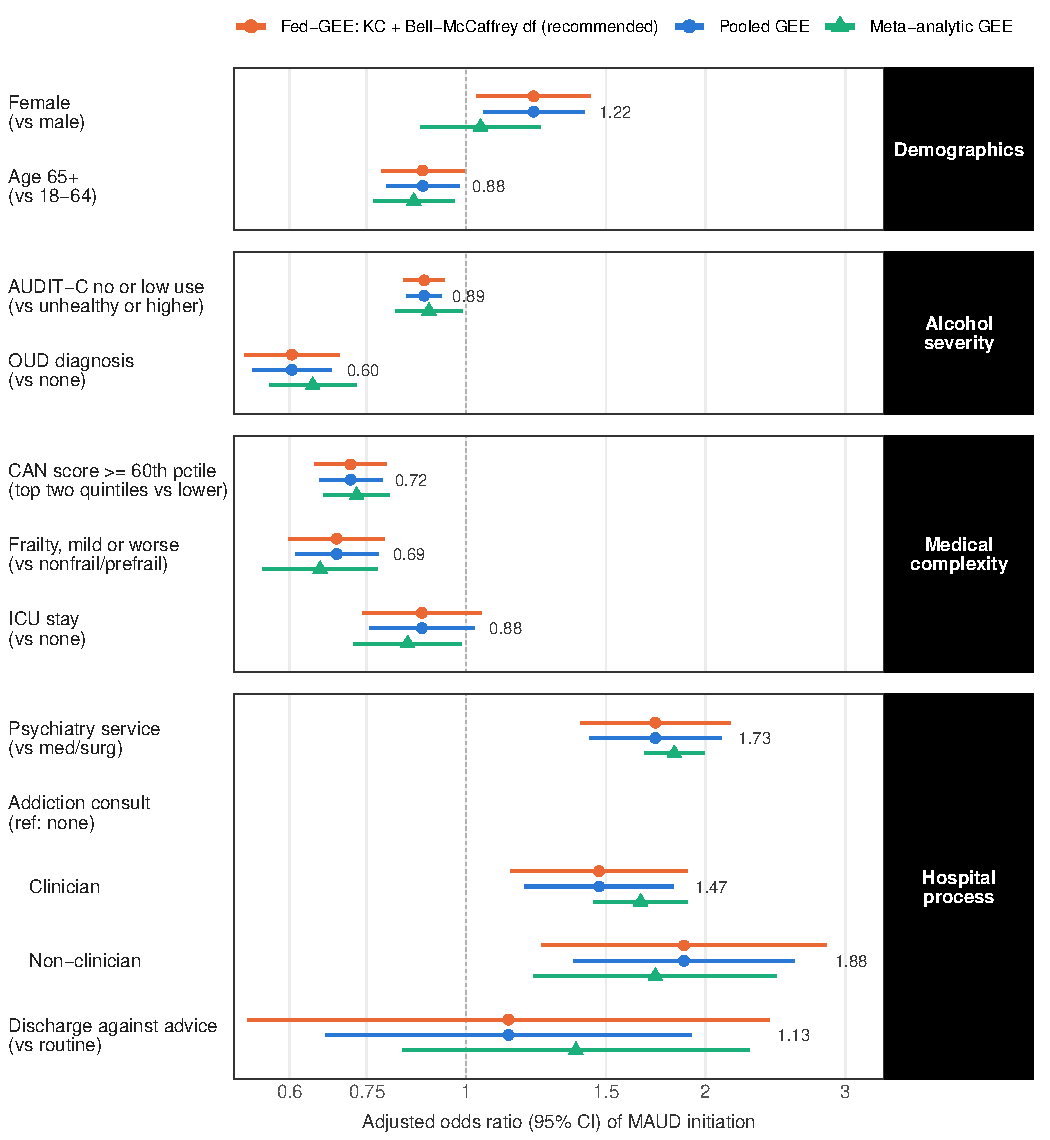
\includegraphics[width=0.9\textwidth]{figures/visn_forest_paper.pdf}
\caption{Adjusted odds ratios and 95\% confidence intervals for MAUD initiation
across 29{,}041 hospitalizations of 18{,}900 Veterans in 18 VISNs, the units of
federation. Fed-GEE uses the score-space Kauermann--Carroll correction with a $t$
reference distribution on Bell--McCaffrey degrees of freedom, computed from the
VISN summaries alone. Pooled GEE uses the uncorrected VISN-clustered sandwich with
a normal reference. Fed-GEE and pooled GEE give identical odds ratios and differ
only in their intervals. Meta-analytic GEE fits a GEE in each VISN and pools the
estimates by inverse-variance weighting. Numeric labels give the Fed-GEE odds
ratio.}
\label{fig:forest}
\end{figure}

\end{document}
